% Template for ICASSP-2017 paper; to be used with:
%          spconf.sty  - ICASSP/ICIP LaTeX style file, and
%          IEEEbib.bst - IEEE bibliography style file.
% --------------------------------------------------------------------------
\documentclass{article}
\usepackage{spconf,amsmath,graphicx}
\usepackage{hyperref}
\usepackage{subcaption}

% Example definitions.
% --------------------
%\def\x{{\mathbf x}}
%\def\L{{\cal L}}

% Title.
% ------
\title{Multi-modal Object Recognition using RGB-D}
%
% Single address.
% ---------------
\name{Khoi-Nguyen Mac}
\address{University of Illinois at Urbana-Champaign}
%
% For example:
% ------------
%\address{School\\
%	Department\\
%	Address}
%
% Two addresses (uncomment and modify for two-address case).
% ----------------------------------------------------------
%\twoauthors
%  {A. Author-one, B. Author-two\sthanks{Thanks to XYZ agency for funding.}}
%	{School A-B\\
%	Department A-B\\
%	Address A-B}
%  {C. Author-three, D. Author-four\sthanks{The fourth author performed the work
%	while at ...}}
%	{School C-D\\
%	Department C-D\\
%	Address C-D}
%
\begin{document}
%\ninept
%
\maketitle
%
\begin{abstract}
The abstract should appear at the top of the left-hand column of text, about
0.5 inch (12 mm) below the title area and no more than 3.125 inches (80 mm) in
length.  Leave a 0.5 inch (12 mm) space between the end of the abstract and the
beginning of the main text.  The abstract should contain about 100 to 150
words, and should be identical to the abstract text submitted electronically
along with the paper cover sheet.  All manuscripts must be in English, printed
in black ink.
\end{abstract}
%
\begin{keywords}
One, two, three, four, five
\end{keywords}
%
\section{Introduction and background}\label{sec:intro}
Object recognition is a problem of computer vision, where the objective is to determine objects in an image or video sequence. This task has multiple applications in real life, such as in autonomous vehicles, where pedestrians, stop signs, traffic lights, etc. are automatically recognized, helping the cars react accordingly. It can be used in security systems, such as video surveillance or face recognition.

There are different researches that try to solve this problem. The classical approach is by using hand crafted features. Such features are extracted from images and clustered together such that each cluster represent a specific aspect of the objects. The process's objective is to create a visual dictionary to represent training objects. New objects are classified based on their features, which are extracted in the same manner as training samples, using nearest neighbors approach \cite{lazebnik_bof}. With the advance of technologies and algorithms, solutions for object recognition are gradually shifting to deep learning methods, where extracted features are machined-based instead of hand-crafted-based, i.e. features are understandable from computer's perspective instead of human. There are several network architectures, started by AlexNet that won the ImageNet challenge and set the new face for object recognition. Some networks recently such as VGG Net \cite{Simonyan2014_vgg}, GoogleNet \cite{googlenet}, and ResNet \cite{resnet} are boosting the architecture complexity and achieving state-of-the-art performance.

Color images suffer from numerous problems, such as inconsistent lighting condition, noisy background data, etc. that reduce system's robustness. Such problems can be solved by using depth information, since depth images contain more information about the shape of objects and ignore patterns on the surface. Therefore, depth images have higher consistency among objects from the same category. In addition, depth cameras are getting more popular therefore such images are easily obtainable.

In this project, I propose to reproduce Eitel et al. paper ``Multimodal deep learning for robust RGB-D object recognition'' \cite{Eitel2015} to build an object recognition system that combines color and depth information to improve accuracy, implemented using Google's TensorFlow \cite{tensorflow2015-whitepaper}. Depth information in converted into RGB images and fed in a branch of the network along side with normal color information. They are then fused and recomputed to produced the final results.
\section{Dataset}\label{sec:dataset}

\begin{figure*}
	\centering
    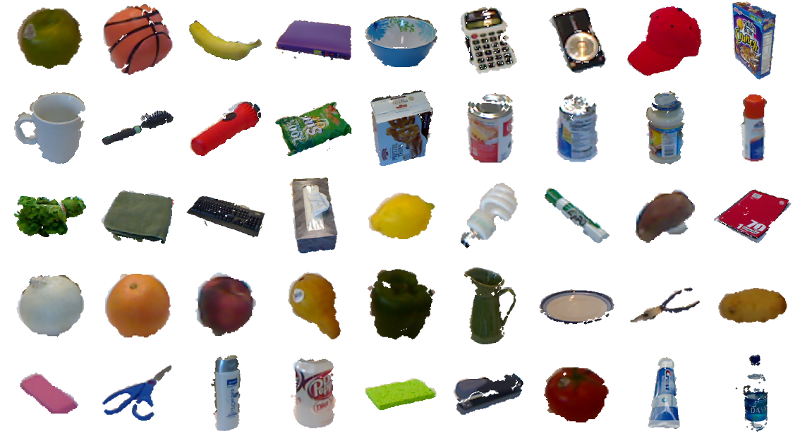
\includegraphics[width=0.8\textwidth]{images/rgbd_dataset}
    \caption{University of Washington's ``RGB-D object dataset''}
    \label{fig:rgb_dataset}
\end{figure*}

In this project, I use ``RGB-D object dataset'' from University of Washington [ref???]. The dataset contains 200,000 samples (each is a collection of color and depth images, and a mask for background removal) of 300 household objects, divided into 51 categories (Figure \ref{fig:rgb_dataset}). Samples from the original dataset are recorded, synchronized, and aligned at the framerate of 30Hz and resolution of $640 \times 480$. However, I use a modified version of the dataset (also provided with the original one), where the objects are localized and cropped out. Each object is recorded on a turntable with three different camera viewpoints: low, middle, and high (Figure \ref{fig:apple_3_viewpoints}).

\begin{figure}
	\centering
	\begin{subfigure}[b]{0.3\linewidth}
	    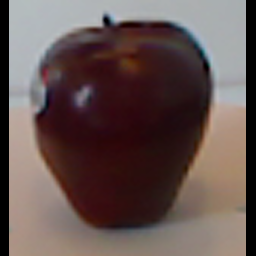
\includegraphics[width=\textwidth]{images/apple_1_1_1_crop.png}
    	\caption{}
	\end{subfigure}
    \begin{subfigure}[b]{0.3\linewidth}
	    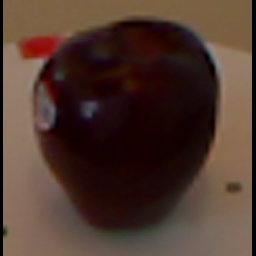
\includegraphics[width=\textwidth]{images/apple_1_2_1_crop.png}
    	\caption{}
	\end{subfigure}
    \begin{subfigure}[b]{0.3\linewidth}
	    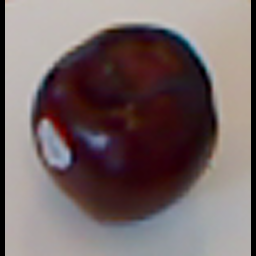
\includegraphics[width=\textwidth]{images/apple_1_4_1_crop.png}
    	\caption{}
	\end{subfigure}
    \\
    \begin{subfigure}[b]{0.3\linewidth}
	    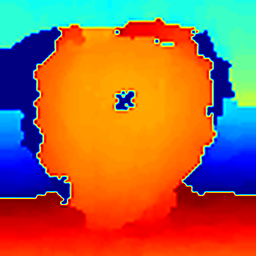
\includegraphics[width=\textwidth]{images/apple_1_1_1_depthcrop.png}
    	\caption{}
	\end{subfigure}
    \begin{subfigure}[b]{0.3\linewidth}
	    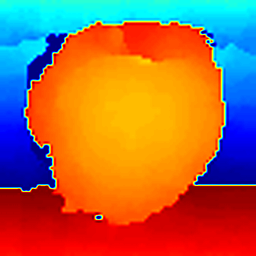
\includegraphics[width=\textwidth]{images/apple_1_2_1_depthcrop.png}
    	\caption{}
	\end{subfigure}
    \begin{subfigure}[b]{0.3\linewidth}
	    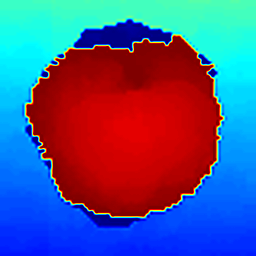
\includegraphics[width=\textwidth]{images/apple_1_4_1_depthcrop.png}
    	\caption{}
	\end{subfigure}
    \caption{Color and (visualized) depth images of an apple from 3 different camera viewpoints.}
    \label{fig:apple_3_viewpoints}
\end{figure}

University of Washington provides another dataset for evaluation. This dataset is constructed as the subset of the original one, keeping one sample out of every five. Samples in this set also have their backgrounds removed. The evaluation set comes with a list of 10 trial, each of which is a split of the dataset for evaluation. For each trial, one object per category is selected for validation, leaving the other objects of the same class for training. Since there are 300 objects and 51 categories, there are 51 objects for evaluation and 249 for training. For the sake of simplicity, I use only the first trial throughout this project's experiments.
\section{Method}\label{sec:method}

%-------------------------------------------------------------------------------------------------------
\subsection{Network architecture}\label{subsec:architecture}
Since the dataset we use is lightweight, containing only 200,000 samples, it is essential to reuse pretrained weights from other network because training from scratch with small dataset would likely result in network overfitting and poor results on test data. As proposed in the paper, AlexNet is inherited in this project. However, this network only accepts inputs with three channels (e.g. RGB images), therefore it can only works with color images instead of depth maps. To bypass this issue, depth maps are colorized in the preprocessing step to convert the data from 1D to 3D. More information about this is discussed in Section \ref{subsec:preprocessing}.

Figure \ref{fig:architecture} illustrates the network's architecture, which can be broken into three networks: one for color-based classification, a network for depth-based classification, and one for fusion that combines the two single-modality streams into a final classification result. Architectures of single stream networks are inherited from AlexNet. However, the final fully connected layer (fc8) from the original network is only used for training single stream networks separately. To fuse them, that classification layer is replaced with two different ones: one for concatenating output from the two streams and one fully connected layer for classifying.

\begin{figure}
	\centering
    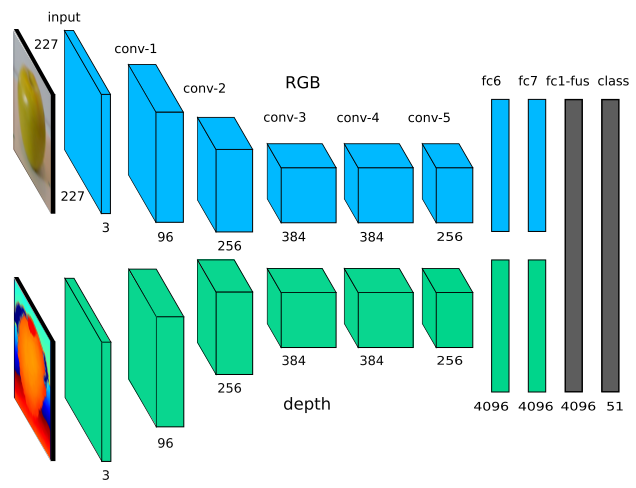
\includegraphics[width=\linewidth]{images/architecture}
    \caption{Fusion network architecture.}
    \label{fig:architecture}
\end{figure}

%-------------------------------------------------------------------------------------------------------
\subsection{Preprocessing}\label{subsec:preprocessing}
There are three primary steps in preprocessing: background removal, resizing, and depth colorization. The first step is straightforward as the mask for each sample is provided with the dataset. However, to test the effect of background removal, I also create another version of prepocessed data with background intact. 

For resizing, the images are rescaled to the shape of $256 \times 256$ although the network receives inputs of dimension $227 \times 227$. This is because we want to remove the mean image of original AlexNet, whose size is $256 \times 256$. After that, the images are randomly cropped to the size of $227 \times 227$ to produce jittering during training. To ensure the shape are not distorted, the images are scaled along the their longer side, the other side is padded with zero (color) and duplicated with boundary (depth), as showed in Figure \ref{fig:apple_3_viewpoints}. However, this does not affect if we remove background from the images.

The third step is to colorize depth. Depth sensors like the Xbox Kinect only give a single-channel intensity image proportional to the distance from the sensor. By converting depth images into three-channel data, we can treat them as images and feed into AlexNet (or other pretrained image recognition networks). Although there are different ways to colorize depth maps, jet colorization is proven superior in term of boosting system’s performance [ref???].

%-------------------------------------------------------------------------------------------------------
\subsection{Network training}\label{sec:training}
The training process in divided into two different phases: (1) training the stream networks and (2) training the fusion network. Suppose that we have the dataset
\begin{equation}
	\mathcal{D} = \left\{ \left(\mathbf{x}^1, \mathbf{d}^1, \mathbf{y}^1\right), ..., \left(\mathbf{x}^N, \mathbf{d}^N, \mathbf{y}^N\right) \right\}
\end{equation}
where $\mathbf{x}^i$ is a RGB image, $\mathbf{d}^i$ is a depth image, and $\mathbf{y}^i$ is a label in the form of
\begin{align}
	\label{equ:label}
	\mathbf{y}^i &= (y_1^i, y_2^i, ..., y_k^i, ..., y_{M}^i)^\top \\
	\text{where} \qquad y_k^i &= 
	\begin{cases}
	1, & \mathbf{x}^i \text{ and } \mathbf{d}^i \text{ belong to class } k\\
	0, & \text{otherwise}
	\end{cases}
\end{align}
where $M$ is the number of classes. The data are fed into the first training phase and then the second one.

\subsubsection{Training the stream networks}
Let $g^I(\mathbf{x}^i; \theta^I)$ be the representation for the color image $\mathbf{x}^i$ of the last fully connected layer from stream networks (\textit{fc7}) of AlexNet, where $\theta^I$ is the parameter. Similarly, we have $g^D(\mathbf{d}^i; \theta^D)$ for the depth image $\mathbf{d}^i$. Since we initialize the stream networks with pretrained weights, $\theta^I$ and $\theta^D$ are known. The weights $\mathbf{W}^I$ and $\mathbf{W}^D$ for RGB and depth streams are trained by solving
\begin{align}
	\min_{\mathbf{W}^I,\theta^I} &= \sum_{i=1}^N \mathcal{L} \left( \text{softmax}\left(\mathbf{W}^I g^I \left(\mathbf{x}^i; \theta^I\right), \mathbf{y}^i\right)\right), \\
	\min_{\mathbf{W}^D,\theta^D} &= \sum_{i=1}^N \mathcal{L} \left( \text{softmax}\left(\mathbf{W}^D g^D \left(\mathbf{d}^i; \theta^D\right), \mathbf{y}^i\right)\right),
\end{align}
where softmax function is
\begin{equation}
	\text{softmax}(z) =\frac{e^z}{\lVert z \rVert_1}
\end{equation}
and the loss is
\begin{equation}
	\mathcal{L}(x,y) = -\sum_k y_k \log s_k.
\end{equation}
This loss function is actually the ``categorical crossentropy'' function, which is commonly used in neural networks.

\subsubsection{Training the fusion network}
After acquiring $\mathbf{W}^I$ and $\mathbf{W}^D$, we discard the softmax layers (\textit{fc8}) and concatenate the last responses of the two streams: $g^I(\mathbf{x}^i; \theta^I)$ and $g^D(\mathbf{d}^i; \theta^D)$ and feed them through the additional fusion layer (\textit{fc1\_fus})
\begin{equation}
	\mathcal{F} = f\left(\left[g^I(\mathbf{x}^i; \theta^I); g^D(\mathbf{d}^i; \theta^D)\right]; \theta^F\right)
\end{equation}
where $\theta^F$ is the parameters of this layer. We can train this layer with a similar manner as in the previous training phase:
\begin{equation}
	\min_{\mathbf{W}^F,\theta^I, \theta^D, \theta^F} = \sum_{i=1}^N \mathcal{L} \left( \text{softmax}\left(\mathbf{W}^F \mathcal{F}, \mathbf{y}^i\right)\right)
\end{equation}

Note that in this phase, the weights trained from the previous one are kept unchanged. Only the weights of the fusion network are optimized.

\subsubsection{Minimizer}

\section{Experimental results}\label{sec:experiments}
\section{Conclusions}\label{sec:conclusions}

In this project, I build a system that can recognize objects using both color and depth information at the same time using TensorFlow. A surprising result is depth information always produce higher accuracy than color only by a simple preprocessing technique: colormapping. It is suspected that depth images strip off patterns on object's surface and reduce the variance in the system, thus the accuracy is higher. Although the system is overfitting, the results are a starting point for further improvement. 

For future work, more experiments with processed depth data are preferred, rather than using raw information. Some possibilities are using ICP algorithmto construct point clouds from depth maps, applying point cloud voxelization, or synthesizing training data from foreign viewpoints. Since depth maps are proved to carry useful information about objects' shape, it is likely that a system cognition can be built using only the mask for background removal. Last but not least, it is promising to try a reversed process from depth colorization, i.e. building a network using only one dimensional depth data.

\vfill\pagebreak

\section{REFERENCES}
\label{sec:refs}

List and number all bibliographical references at the end of the
paper. The references can be numbered in alphabetic order or in
order of appearance in the document. When referring to them in
the text, type the corresponding reference number in square
brackets as shown at the end of this sentence \cite{C2}. An
additional final page (the fifth page, in most cases) is
allowed, but must contain only references to the prior
literature.

% References should be produced using the bibtex program from suitable
% BiBTeX files (here: strings, refs, manuals). The IEEEbib.bst bibliography
% style file from IEEE produces unsorted bibliography list.
% -------------------------------------------------------------------------
\bibliographystyle{IEEEbib}
\bibliography{strings,refs}

\end{document}
